
\chapter{New system}
The most important change we plan to make is to gather all the existing system under one site. Since Innsida already exists and contains external links to other systems like Student Web, It’s Learning, Email etc., it would be natural to use it as our base. Our new system will work as the front-end and FS (Felles Sudentsystem) will continue to serve as the back-end. All the functionality that is today covered by different systems will be moved to tabs, that will be accessible through every page in the system. Users will no longer wait too long for updates and they will have to log in once to access the system as a whole. We assume that it is secure enough to log in only via feide using username and password.

\section{News feed - main page}
Innsida as it is now consists of all the systems used by NTNU, but redundancy and confusing structure makes it hard to comprehend. News feed is the biggest part of the page, and we see it as a useful field, but its content in today's system is not consisting of important information and it's not systematized. We would like to keep the news feed as the only field on the main page, divided into subfields. Each subfield would have different function: one for general news, one for notifications for student taking specific courses (like warnings about closing deadlines), news sent by a faculty in which they belong, and possibly more. This way users will be alerted when something important is going on. Figure \ref{fig:home} presents an example sketch of the whole system. 

\section{Email}
Users are already provided with Microsoft Outlook as Email system. It is a standard solution to use an existing service for that, and we intend to keep with a few changes. As it happens a lot in today's system that user has to log in two times to access different services (for example Innsida first, then Outlook), we would like to have Outlook as an underlying system accessed via a tab on the main page. That way logging in would be no issue, and other services would be available at any time. Figure \ref{fig:email} shows BPMN model for sending an email.

\begin{figure}[h]
\centering
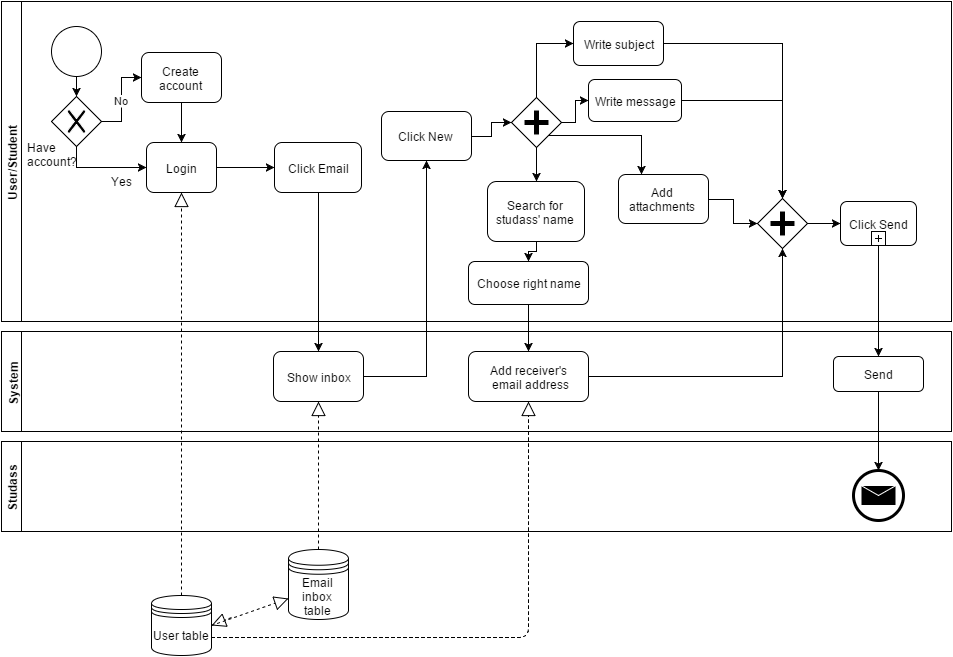
\includegraphics[width=\linewidth]{sec/Send_email_to_studass.png}
\caption{Sending email to studass}
\label{fig:email}
\end{figure}
\newpage

\section{It's Learning}
As we see it It's Learning provides little to no functionality needed in the system. Message system is already taken care of by Email system, and many courses use other systems for assignment evaluation and storing other important files (like TDT4120 has a simple website). Link to the library is also unnecessary - it can be accessed via ntnu.no. Some of the courses still use It's learning, which means that we need an alternative that covers functionality that is actually used. We were thinking of making a tab under main page called "Courses", where all  the courses a user has something to do with at the moment (student, lecturer etc.) are listed. There would be possibility to deliver an assignment or evaluate it, depending on the kind of user. It would be also possible to deliver assignments in a group using participant overview (if teacher allows it). Important information like closing deadlines or new evaluation are supposed to be displayed in the feed on main page. A simple file system would be also provided. On top of that, students may easily add or remove courses directly from the list, given the deadline for that hasn't passed. This way one doesn't have to use two systems for that (i.e. It's Learning and Student Web), log in twice or wait for daily update. Figure \ref{fig:regview} shows the approach.

\begin{figure}[h]
\centering
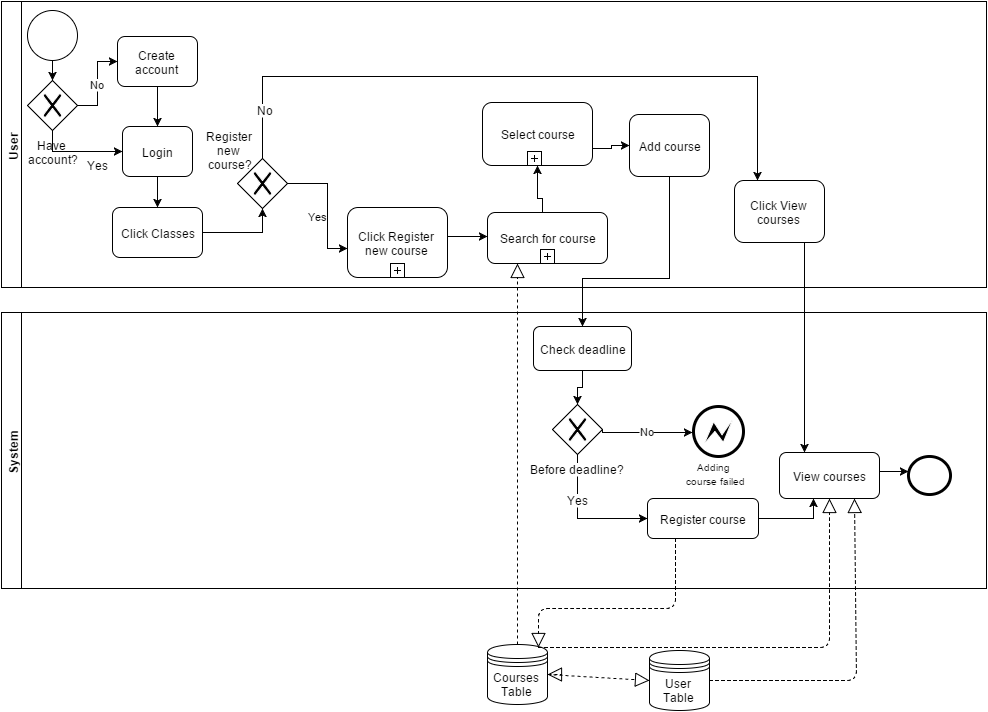
\includegraphics[width=\linewidth]{register_view_courses.png}
\caption{Register or view course}
\label{fig:regview}
\end{figure}
\newpage

\section{Student Web}
Since Student web is mostly a front-end to FS, it should be no problem to replicate the utility you can find on this site in our system. We want to keep some services provided by it, where editing course list would be done as described in section 3.3. All the functionality that is course related will be accessed via "Courses" tab. There will be fields for past courses and actual courses. The last essential function that needs to be covered is semester fee payment. Student web's existing solution for that can be included in a tab called "Payments".

\subsection{Past courses}
For students, past courses will display courses that one has taken that have complaint deadline expired. It shows a list consisting course names, assignment statuses, assignment grading (if they count for the final grade), exam grades and calculated final grade. It will be possible to display the list in study plan view, with specified semesters and years. This approach makes it easy to have a clear overview and access all the information relevant to courses in one place. This kind of overview also makes it easier for students to choose future courses.
\subsection{Actual courses}
This section displays courses taken in current semester, along with assignment statuses (grades) and exam date. If a student has taken an exam in a course and is waiting for evaluation, the course will be displayed as pending. After receiving exam grade, final grade will we calculated, and course will stay in the subsection until complaint deadline has passed. As for past courses, overview is clear and access is easy.  

\section{Eksamensweb}
Eksamensweb is a service accessible only for IME students, while others faculties each have a site including complaint form. In our solution students can complain directly through the main system in Actual courses subsection. As long as the grade has been calculated and deadline hasn't passed, there is Complain button next to it. System checks which faculty courses belongs to, so that user is redirected to right form. The form is partially filled in based on information from the system, so that grade complaining is as easy and intuitive as possible. Student can also be sure that all the information is correct. Issuing a complaint is showed in figure \ref{fig:complaint}.  


\begin{figure}[h]
\centering
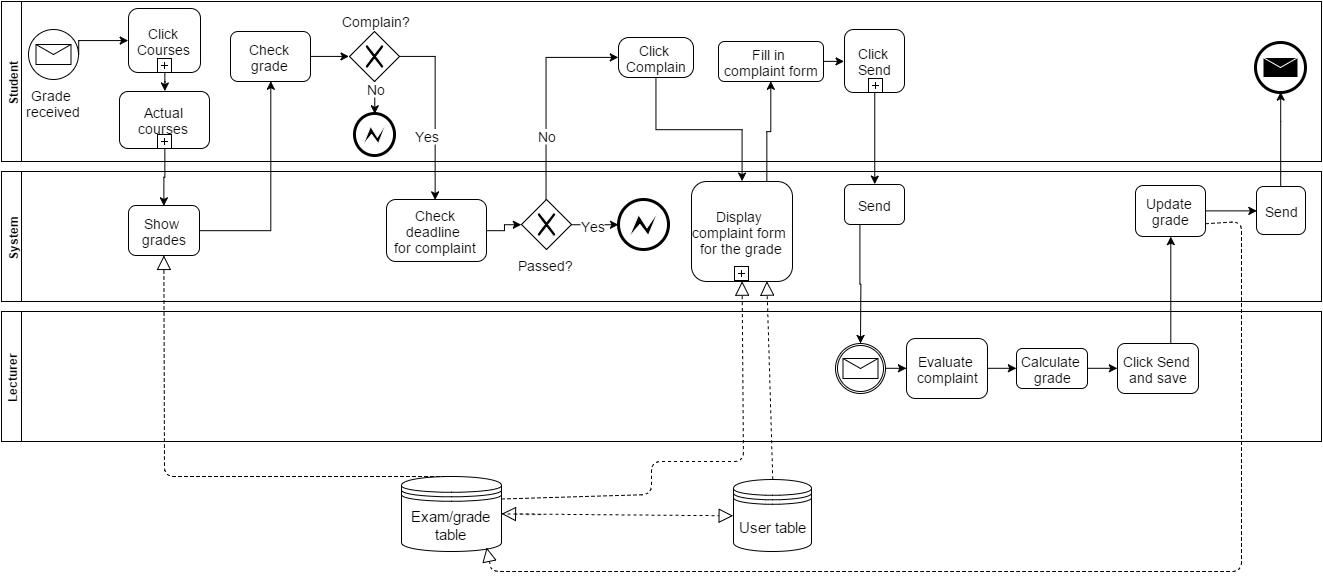
\includegraphics[width=\linewidth]{grade_complaint.png}
\caption{Grade complaint (given user is logged in)}
\label{fig:complaint}
\end{figure}
\newpage

\begin{figure}[h]
\centering
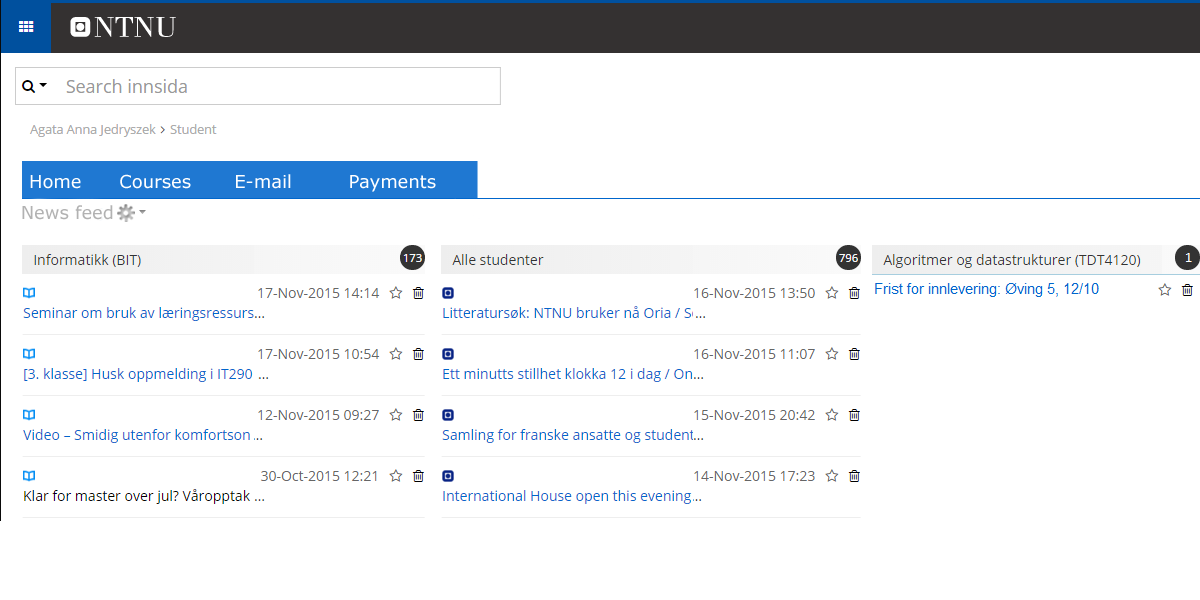
\includegraphics[width=\linewidth]{home.png}
\caption{Sketch of possible solution - main page}
\label{fig:home}
\end{figure}
\newpage


